%
%  untitled
%
%  Created by Byron Wallace on 2013-11-13.
%  Copyright (c) 2013 . All rights reserved.
%
\documentclass[]{article}

% Use utf-8 encoding for foreign characters
\usepackage[utf8]{inputenc}

% Setup for fullpage use
\usepackage{fullpage}

% Uncomment some of the following if you use the features
%
% Running Headers and footers
%\usepackage{fancyhdr}

% Multipart figures
%\usepackage{subfigure}

% More symbols
%\usepackage{amsmath}
%\usepackage{amssymb}
%\usepackage{latexsym}

% Surround parts of graphics with box
\usepackage{boxedminipage}

% Package for including code in the document
\usepackage{listings}

% If you want to generate a toc for each chapter (use with book)
\usepackage{minitoc}

% This is now the recommended way for checking for PDFLaTeX:
\usepackage{ifpdf}

%\newif\ifpdf
%\ifx\pdfoutput\undefined
%\pdffalse % we are not running PDFLaTeX
%\else
%\pdfoutput=1 % we are running PDFLaTeX
%\pdftrue
%\fi

\ifpdf
\usepackage[pdftex]{graphicx}
\else
\usepackage{graphicx}
\fi
\title{Noisy Tree LDA}
%\author{  }

\date{2013-11-13}

\begin{document}

\ifpdf
\DeclareGraphicsExtensions{.pdf, .jpg, .tif}
\else
\DeclareGraphicsExtensions{.eps, .jpg}
\fi

\maketitle


%\begin{abstract}

%\end{abstract}

\section{Introduction}

We consider scenarios in which we observe noisy samples drawn from tree-structured data. More specifically, this problem is motivated by domains for which expert ontologies exist. In such cases, observations may be associated with nodes at different levels in said ontology.

\begin{figure}[h!]
  \centering
    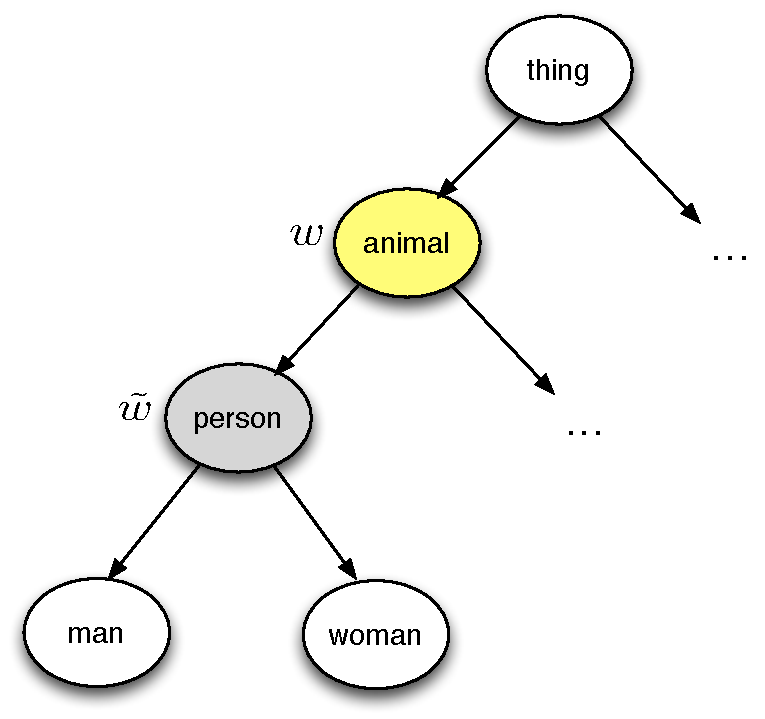
\includegraphics[scale=.5]{../figures/ontology-observed.pdf}
  \caption{The noisy LDA scenario. Nodes are terms in an expert ontology. We assume that we have observed term $w$ while the `true' (unobserved) term is $\tilde{w}$.}
\end{figure}

\section{A `Noisy Structured LDA' Topic Model}	

\begin{eqnarray}
 \theta &\sim& \textrm{Dir}(\alpha) \\
  \beta_z &\sim& \textrm{Dir}({\eta})  \\
  z &\sim& \textrm{Mult}(\theta) \label{eq:true_z}\\
  w|z &\sim& \textrm{Mult}(\beta_z) \\
  \tilde{w}|w,\mathcal{O} &\sim& \lambda(w, \mathcal{O})
\end{eqnarray}


We will denote the expert ontology by $\mathcal{O}$ and latent distributions over terms $\in \mathcal{O}$ by $z$ -- these can be viewed as topics. Further, we will denote the (corpus-wide) distribution over topics by $\theta$, and the conditional distribution over terms given component $z$ by $\theta_z$ (for all topics $z$). We will then assume that a given latent `true' term $w$ is drawn from the underlying structure $\mathcal{O}$. But rather than observing this directly, we observe a token $\tilde{w}$ drawn conditioned on $w$, i.e., a `noisified' $w$. Intuitively, this can be viewed as allowing for variation in the process of assigning terms to instances (citations, patients, etc.) on behalf of domain experts; this variation is constrained by the underlying structure.

The biggest question, then, is how to model $\tilde{w}|w,\mathcal{O}$ (i.e., $\lambda(w, \mathcal{O})$). Intuitively, this should quantify the probability of observing $w_j$ given its position in $\mathcal{O}$ vis-a-vis that of $w$. So then the further (w.r.t. $\mathcal{O}$) $w_j$ is from $w$, the less likely $w_j$. One obvious way of realizing this would be to place a multinomial over the ontology vocabulary:

\begin{equation}
	\tilde{w}|w,\mathcal{O} \sim \textrm{Mult}(\gamma_0, \gamma_1, ... , \gamma_N)
\end{equation}

\noindent Where the $\gamma$ terms are set to reflect some notion of (normalized) distance. 

In any case, an important assumption here is that the underlying `topics' are sparse, i.e., are associated with a few key terms in the ontology. This sparsity will need to be enforced for the $\theta$ parameters in Equation \ref{eq:true_z}.



%\bibliographystyle{plain}
%\bibliography{}
\end{document}
